\chapter{La détection des anomalies}



\section{Description de la détection des anomalies dans liens}

La détection des anomalies dans les délais des liens passe par deux étapes principales. La première étape consiste à préparer les traceroutes. Quant à la deuxième étape, elle sert à calculer une référence pour ensuite comparer les nouvelles valeurs avec la valeur de référence. Cette  référence représente un intervalle de valeurs des RTTs différentiel ou un intervalle de confiance, toute nouvelle valeur de RTT est comparée avec l'intervalle de confiance et suite à cette comparaison, on caractérise le changement par rapport à la référence.  

\subsection{Vue générale du processus de la détection}

 La figure 	\ref{fig:process-detection} reprend le processus de la détection des anomalies dans le délais d'un lien. On distingue les deux étapes principales : la préparation des traceroutes et l'exploitation des données issues de l'étape de la préparation.  Dans chacune des étapes, on distingue un succession d'opérations. 
 
 L'objectif de l'étape de préparation des traceroutes est de traiter chaque traceroute, indépendamment des autres traceroutes. Toutefois, ces traceroutes sont regroupés par période, où une période est une durée marquée par un début et une fin. En ce qui concerne la deuxième étape, elle exploite les données de la première étape pour identifier les liens et les différents changements que l'ont subi.
  
\begin{figure}[H]
	\centering
	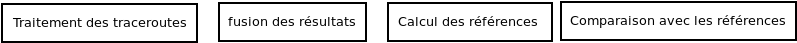
\includegraphics[width=1\linewidth]{illustrations/process-detection}
	\caption{Le processus de l'analyse des délais d'un lien.}
	\label{fig:process-detection}
\end{figure}

\subsection{Préparation des données}
 A l'étape de la préparation des traceroutes, on distingue trois opérations, premièrement c'est l'élimination des données inutiles dans un traceroute, voire le traceroute même s'il a échoué. Deuxièmement, c'est l'identification des liens topologiques et leurs caractérisation. Enfin, c'est la fusion des données si c'est nécessaire. 
 
\paragraph{L'élimination des données inutiles}  Un traceroute est sauvegardé en étant un object JSON, la figure \ref{annexe:traceroute-attributes} décrit les attributs qu'un traceroute peut contenir. D'une part, il y a les attributs obligatoires dont chaque traceroute doit révéler. D'autre part, il existe les attributs optionnels.  La conservation de tel ou tel attribut dépend de l'objectif pour lequel un traceroute est analysé.  

\paragraph{Vérification de la validation des données utiles} Les données utiles dans l'analyse des délais doivent être validées suivant les objectifs spécifiques prédéfinis. Etant donné que l'analyse des délais ne concerne pas les réseaux informatiques privés, les adresses IP privées sont éliminées. Comme une sonde Atlas peut recevoir jusqu'à trois signaux différents pour un saut donné, chaque signal doit reprendre un RTT et une adresse IP source du signal. Le RTT doit être valide; positif non nul.
 
\subsection{Exploitation des données}

\section{Application de l'algorithme de la détection}


